\documentclass[border=6pt]{standalone}
\usepackage{fontspec}
\defaultfontfeatures{Ligatures=TeX}
\setmainfont{Palatino Linotype}
\usepackage{tikz}
\usetikzlibrary{arrows.meta, positioning, calc, shapes.geometric, fit,
                backgrounds, decorations.pathmorphing}
\definecolor{casink}{HTML}{1A1A22}
\definecolor{casaccent}{HTML}{6B3F8C}
\definecolor{casmuted}{HTML}{8A8A94}
\definecolor{caswash}{HTML}{F0ECF4}

\tikzset{
  casnode/.style={
    draw=casink, line width=0.5pt, rounded corners=1.2pt,
    fill=caswash, inner sep=3.2pt, font=\small, minimum height=6.5mm,
    align=center},
  casdomain/.style={
    casnode, minimum width=34mm, font=\small\bfseries},
  casflow/.style={
    -{Stealth[length=2.1mm,width=1.6mm]}, draw=casink, line width=0.55pt},
  casfeedback/.style={
    -{Stealth[length=2.1mm,width=1.6mm]}, draw=casmuted, line width=0.5pt,
    dashed, dash pattern=on 1.6pt off 1.4pt},
  casinvol/.style={
    {Stealth[length=1.8mm,width=1.4mm]}-{Stealth[length=1.8mm,width=1.4mm]},
    draw=casaccent, line width=0.5pt},
  caslabel/.style={font=\scriptsize, text=casmuted},
  cascap/.style={font=\scriptsize\itshape, text=casink},
}

% Every figure in this book uses the same wrapper so the list of figures and
% the numbering stay consistent.
\newcommand{\casfig}[3]{%
  \begin{figure}[htbp]
  \centering
  #2
  \caption{#3}\label{fig:#1}
  \end{figure}%
}

\begin{document}

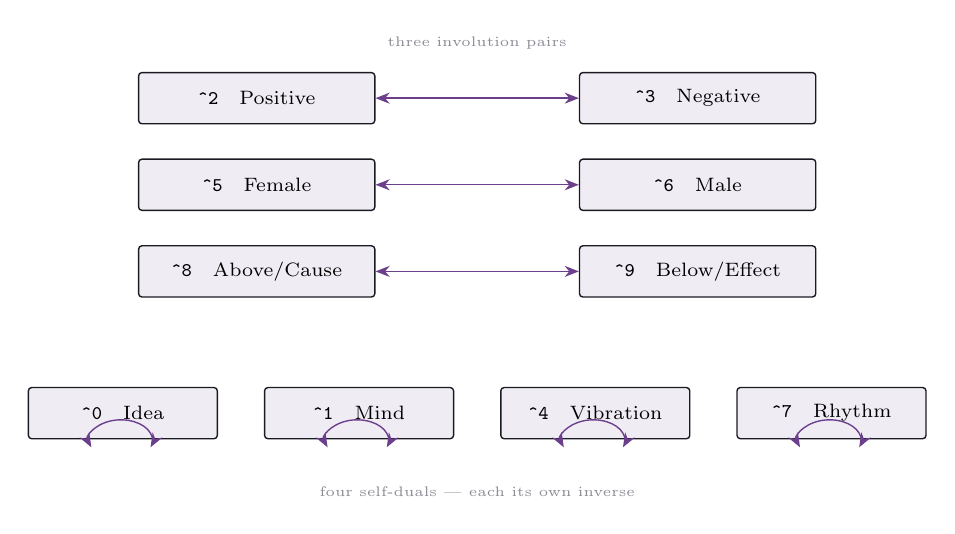
\begin{tikzpicture}
  % Involution pairs placed FACING each other, which is the structural claim.
  % A ring layout would put them side by side and say nothing.
  \foreach \i/\sym/\name in {0/2/Positive, 1/5/Female, 2/8/{Above/Cause}} {
    \node[casnode, minimum width=30mm, font=\scriptsize]
      (L\i) at (0, -\i*11mm) {\texttt{\^{}\sym} \; \name};
  }
  \foreach \i/\sym/\name in {0/3/Negative, 1/6/Male, 2/9/{Below/Effect}} {
    \node[casnode, minimum width=30mm, font=\scriptsize]
      (R\i) at (56mm, -\i*11mm) {\texttt{\^{}\sym} \; \name};
  }
  \foreach \i in {0,1,2} { \draw[casinvol] (L\i) -- (R\i); }

  \node[caslabel, font=\tiny] at (28mm, 7mm) {three involution pairs};

  % the four self-duals
  \foreach \i/\sym/\name in {0/0/Idea, 1/1/Mind, 2/4/Vibration, 3/7/Rhythm} {
    \node[casnode, minimum width=24mm, font=\scriptsize]
      (S\i) at (\i*30mm - 17mm, -40mm) {\texttt{\^{}\sym} \; \name};
    \draw[casinvol] (S\i.south) ++(-4mm,-1mm)
      arc (200:-20:4mm and 2.6mm);
  }
  \node[caslabel, font=\tiny, align=center] at (28mm, -50mm)
    {four self-duals --- each its own inverse};
\end{tikzpicture}

\end{document}
